\chapter{Solución}

Una vez nos hemos situado en el contexto en el que se ubica este proyecto, y hemos expuesto los requisitos a cumplir y las herramientas necesarias para llegar a las metas planteadas, nos adentramos a explicar en este capitulo las soluciones utilizadas para llegar a buen puerto.\\

\section{Estructura general}

Como primer problema se presentó decidir cuál de los dos ordenadores que necesitamos para la conexión WebRTC seria el que realizaría la llamada y en que momento del flujo. Este no es un problema trivial, ya que la selección de uno u otro haría que el desarrollo de la aplicación fuese completamente distinto.\\

Se optó por que el par que llevase la batuta de la conexión fuese el ordenador local, ya que este a su vez también es el encargado de  establecer la conexión con el drone. De esta manera tenemos un par que es el que actuará de maestro, estableciendo ambas conexiones en los momentos oportunos.\\

Como ya se comento en la sección \ref{sec:senalizacion} el momento en el que se envía y se recibe cada paquete de información es critico en este sistema de señalización de oferta/respuesta, por lo que el flujo de la comunicación se diseñó y se ha desarrollado como se muestra en la figura \ref{fig:flujodellamada}.\\


\begin{figure}[htb]
\centering
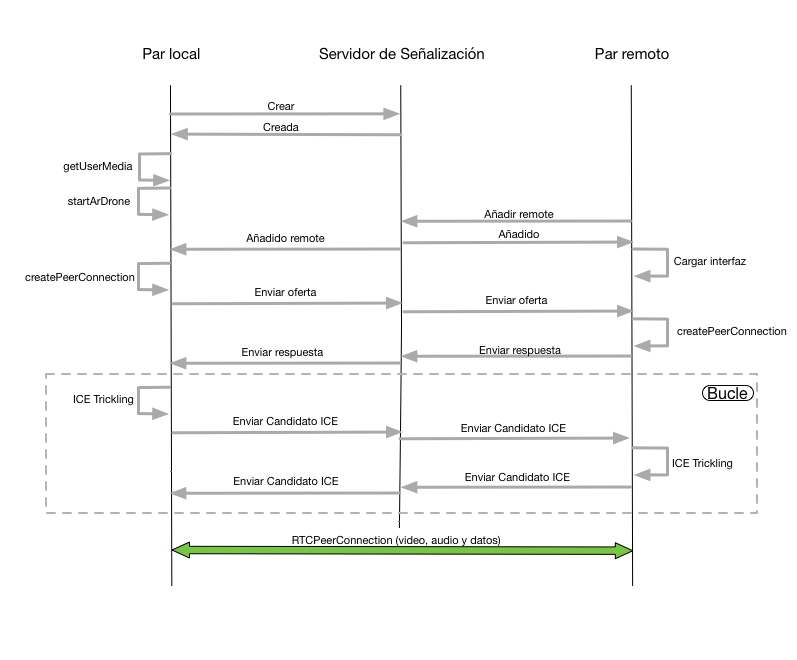
\includegraphics[width=1.1\textwidth]{diagrama_general}
\caption{Flujo de llamada del proyecto}
\label{fig:flujodellamada}
\end{figure}



\section{Conexión con la API del drone}

Para establecer la conexión con el drone se ha utilizado el componente \texttt{ardrone\_server} de JdeRobot. Este componente tiene dos versiones, la componente simulada que es la que hemos instalado en forma de plugin en el simulador Gazebo y la componente real, que se conecta al drone real. Ambas componentes nos ofrecen las mismas interfaces de conexión, por lo que una única configuración de nuestra aplicación bastará para poder trabajar con la versión simulada o la real.\\

En este punto podemos dividir el proyecto en dos partes. Servidor y Cliente. La parte de servidor trataremos básicamente la configuración, y la parte del cliente será la que desarrolla desde cero.\\


\subsection{Servidor}

Los componentes JdeRobot utilizan, como ya hemos visto, interfaces ICE para el intercambio de información del que se ocupan. Los navegadores no tienen capacidad de usar el \emph{middlewre} ICE directamente. Para poder conectarnos con estas interfaces ICE hemos tenido que instalar el plugin ICE for JavaScript, o ICE\-JS. Este plugin nos habilita la opción de conectarnos a estas interfaces directamente desde el navegador usando \emph{websockets}.\\

Aunque estaba disponible la versión 3.6 de ICE\footnote{https://doc.zeroc.com/display/Ice36/Home} la cuál trae en la suite instalado de serie ICE\_JS, hemos usado la versión 3.5, ya que es la versión compatible con la versión más actual de JdeRobot\footnote{http://jderobot.org/Manual-5}. En esta versión ICE\_JS es un plugin a parte el cuál hay que instalarlo descargando el código fuente desde la página de Zeroc\footnote{https://zeroc.com} y compilarlo.\\

Una vez instalado hay que activar este plugin en el servidor. Para ello hay que añadir la siguiente línea en el archivo de configuración del servidor:\\

\begin{lstlisting}[caption=Activación del plugin ICEJS]
# ICE-JS
Ice.Plugin.IceWS=IceWS:createIceWS
\end{lstlisting}

Posteriormente a esto, en el mismo archivo hay que indicarle las direcciones IP y los puertos de cada interfaz de conexión. Cada conexión se corresponderá con un \emph{WebSocket}, y la nomenclatura es la siguiente:\\

\begin{lstlisting}[caption=Formato \emph{endpoints} de los \emph{WebSocket} de ICEJS]
# ICE-JS
:ws -h ip -p puerto
\end{lstlisting}

El servidor tiene hasta un máximo de seis interfaces diferentes a las que te puedes conectar. Cada uno de estas interfaces nos ofrece un servicio diferente. Para nuestro proyecto usaremos cuatro de esas interfaces.

\begin{itemize}
\item \textbf{Pose3D:} Con esta interfaz accedemos a los datos pose del cuadricóptero (x, y, z, h y \emph{quaternion}).
\item \textbf{Navdata:} Esta interfaz nos proporciona los datos de navegación procedentes de los sensores, como la velocidad de las componentes (x, y, z) del drone, altitud, la velocidad del viento, el nivel de batería, etc.
\item \textbf{CMDVel:} Esta interfaz en la que se encarga de recibir las órdenes de movimiento.
\item \textbf{BaseExtra:} Esta interfaz nos da funcionalidades extra como el aterrizaje o el despegue del cuadricóptero.
\end{itemize}

Así pues, esta es la forma final que tiene nuestro archivo de configuración:\\

\begin{lstlisting}[caption=Archivo de configuración]
# Ice-JS
Ice.Plugin.IceWS=IceWS:createIceWS

# Variables de control para ver traceroutes de las conexiones ICE.
#Ice.Trace.Network = 3
#Ice.Trace.Protocol=1


ArDrone.Pose3D.Endpoints=default -h 0.0.0.0 -p 9998:ws -h 0.0.0.0 -p 19000
ArDrone.Pose3D.Name=ardrone_pose3d

ArDrone.RemoteConfig.Endpoints=default -h 0.0.0.0 -p 9997
ArDrone.RemoteConfig.Name=ardrone_remoteConfig

ArDrone.Navdata.Endpoints=default -h 0.0.0.0 -p 9996:ws -h 0.0.0.0 -p 15000
ArDrone.Navdata.Name=ardrone_navdata

ArDrone.CMDVel.Endpoints=default -h 0.0.0.0 -p 9995:ws -h 0.0.0.0 -p 11000
ArDrone.CMDVel.Name=ardrone_cmdvel

ArDrone.Extra.Endpoints=default -h 0.0.0.0 -p 9994:ws -h 0.0.0.0 -p 17000
ArDrone.Extra.Name=ardrone_extra

ArDrone.NavdataGPS.Endpoints=default -h 0.0.0.0 -p 9993
ArDrone.NavdataGPS.Name=ardrone_navdatagps
\end{lstlisting}

A parte de los \emph{endpoints} es también importante configurar correctamente el nombre de cada uno de las interfaces, ya que será necesario para una correcta conexión desde el navegador.\\


\subsection{Cliente}

Una vez configurado el servidor hemos creado el método ArDrone.js, el cuál es el encargado de conectarse y manejar la conexión con el servidor \texttt{ardrone\_server}.\\

Para establecer una comunicación ICE lo primero es crear las variables ICE necesarias. Estas las creamos de la siguiente manera:\\

\begin{lstlisting}[caption=Formato \emph{endpoints} de los \emph{WebSocket} de ICEJS]
// Variable ICE para la conexion
var id = new Ice.InitializationData();
id.properties = Ice.createProperties();
id.properties.setProperty("Ice.Trace.Network", "3"); // Propiedad para tracear la conexion
id.properties.setProperty("Ice.Trace.Protocol", "1"); // Propiedad para tracear la conexion
var communicator = Ice.initialize(id);
\end{lstlisting}

Por si fallase la comunicación ICE se le ha añadido a la variable \emph{id} una propiedad con la que podemos seguir la ruta de la comunicación y detectar en que punto se produce el fallo.\\

Posteriormente es necesario crear una variable, que será la que actuará como \emph{proxy}, por cada interfaz a la que necesitemos conectarnos. Esta es la nomenclatura que debe seguir:\\

\begin{lstlisting}[caption=Nomenclatura de variable que actuará como \emph{proxy}]
var proxy = communicator.stringToProxy("nombre_interfaz:ws -h " + ip + " -p " + "puerto");
\end{lstlisting}

La comunicación con las interfaces se realiza mediante el objeto promesa o \emph{promise}. Este objeto se usa para las comunicaciones asíncronas y se caracteriza por tener tres estados: pendiente, cumplida o rechazada. Cuando una promesa ha sido llamada puede presentar el estado cumplida o rechazada, lo que nos permite llamar al argumento correspondiente y poder actuar en consonancia. De esta manera podemos hacer que métodos asíncronos actúen como métodos sincronos.\\

El núcleo de la conexión con el servidor \emph{ardrone\_server} queda como sigue:\\

\begin{lstlisting}[caption=Nucleo ArDrone]
// base extra connection
var baseextra = communicator.stringToProxy("ardrone_extra:ws -h " + ip + " -p " + baseextraPort);
jderobot.ArDroneExtraPrx.checkedCast(baseextra).then(
    function(ar){
        extraProxy = ar;
        console.log("extraProxy connected: " + ar);
    },
    function(ex, ar){
        console.log("extraProxy NOT connected: " + ex);
    }
);               

// NavData
var basenavdata = communicator.stringToProxy("ardrone_navdata:ws -h " + ip + " -p " + navdataProxyPort);
jderobot.NavdataPrx.checkedCast(basenavdata).then(
    function(ar){
        console.log("navdataProxy connected: " + ar);
        navdataProxy = ar;
        navdataProxy.getNavdata().then(
        function(navdata){
            if (navdata.vehicle == ARDRONE_SIMULATED) {
                virtualDrone = true;
                console.log("virtualDrone = true");
            } else {
                virtualDrone = false;
                console.log("virtualDrone = false");
            }
        },
        function (ex, ar){
            console.log("Fail getNavdata() function: " + ex);
        }
        );
    },
    function (ex, ar){
        console.log("navdataProxy NOT connected: " + ex);
    }        
);        

// CMDVelPrx
var basecmdVel = communicator.stringToProxy("ardrone_cmdvel:ws -h " + ip + " -p " + cmdVelProxyPort);
jderobot.CMDVelPrx.checkedCast(basecmdVel).then(
    function(ar){
        console.log("cmdVelProxy connected: " + ar);
        cmdVelProxy = ar;
    },
    function(ex, ar){
        console.log("cmdVelProxy NOT connected: " + ex);
    }
);             

// Pose3D
var basepose3D = communicator.stringToProxy("ardrone_pose3d:ws -h " + ip + " -p " + pose3DProxyPort);
jderobot.Pose3DPrx.checkedCast(basepose3D).then(
   function(ar){
       console.log("pose3DProxy connected: " + ar);
       pose3DProxy = ar;
        window.po = pose3DProxy;
        resolve("Stuff worked!");
       pose3DProxy.getPose3DData().then(
           function (ar){
               console.log("getPoseDData().");
               pose = ar;
           },
           function(ex, ar){
               console.log("Fail call getPoseDData().");
           });
   },
   function(ex, ar){
       console.log("pose3DProxy NOT connected: " + ex)
   }
);
\end{lstlisting}

En este punto ya estamos conectados con las interfaces del servidor, y por consiguiente, con el drone. Para poder teleoperar el drone hay que crear unas funciones que serán los manejadores. Por un lado hemos creado las funciones de aterrizaje y de despegue. Estas funciones utilizan la interfaz \emph{ardrone\_extra}:\\

\begin{lstlisting}
// extraProxy functions  
function takeoff() {
    extraProxy.takeoff().then(
        function(ar){
            console.log("Take Off.");
        },
        function(ex, ar){
            console.log("Take Off failed.")
        }
     );
}
    
function land() {
        extraProxy.land().then(
        function(ar){
            console.log("Landing.");
        },
        function(ex, ar){
            console.log("Landing failed: " + ex)
        }
     );
}
\end{lstlisting}

Estas son las funciones encargadas de leer los datos de los sensores a través de las interfaces \emph{Navdata} y \emph{Pose3D}:\\

\begin{lstlisting}

function updateNavData() {
    navdataProxy.getNavdata().then(
        function(ar){
            navdata = ar;
            //console.log("updateNavData()");
        },
        function (ex, ar){
            console.log("Fail getNavdata() function." + ex)
        }        
    );    
}

function updatePose(){
    pose3DProxy.getPose3DData().then(
            function (ar){
                pose=ar;
                //console.log("getPose3DData. ")
            },
            function(ex, ar){
                console.log("Fail call getPoseDData(): " + ar2);
            });   
}

\end{lstlisting}


Llamando a estas funciones periódicamente tenemos actualizados los datos de navegación del procedentes de los sensores: brújula, posición, velocidad, altitud...\\

Para poder teleoperar el drone se ha implementado una función que es la encargada de enviarle las órdenes de movimiento. \\

\begin{lstlisting}

function sendVelocities () {
    cmdVelProxy.setCMDVelData(cmd).then(
        function(ar){
          //console.log("sendVelocities.");
        },
        function(ex, ar){
          console.log("sendVelocities failed.")
        }
    );
}

\end{lstlisting}

Dónde la variable \emph{cmd} contiene los parámetros que necesita el drone para moverse. Esta variable es una variable CMDVel de JdeRobor y tiene esta estructura:\\

\begin{lstlisting}

var cmd = new jderobot.CMDVelData; 
cmd.linearX=0.0;
cmd.linearY=0.0;
cmd.linearZ=0.0;
cmd.angularZ=0.0;
cmd.angularX=0.0;
cmd.angularY=0.0;

\end{lstlisting}


\subsubsection{getUserMedia}

La interfaz que no hemos implementado de las que nos ofrece el servidor \texttt{ardrone\_server} es la interfaz \emph{cameraserver}. Esta interfaz se encarga de recoger las imágenes de la cámara integrada en el drone. Para tener una imagen con mas resolución y que nos permita visualizar con mayor calidad se ha optado por colocar una cámara a bordo y acceder a ella con las herramientas que nos suministra WebRTC.\\

Esta camara se conecta a nuestro ordenador local a través de una conexión USB. Camara y MiniPC vana a bordo del drone. Como WebRTC aún no es una norma, para acceder a la cámara desde cualquier navegador debemos crear una variable que sea compatible con todos los que tengan implementado las APIs de WebRTC. Para ello hay que añadirle los prefijos correspondientes de cada navegador:\\


\begin{lstlisting}
navigator.getUserMedia = navigator.getUserMedia || navigator.webkitGetUserMedia || navigator.mozGetUserMedia;
\end{lstlisting}


Acceder a la cámara a con \emph{GetUserMedia} se hace a través de una función que admite dos llamadas de vuelta o \emph{callback}. Uno de ellos es el callback de éxito, y el segundo el de error. Según sea de exitosa el acceso a la cámara se llamara a una función u otra. Si nos devuelve éxito se llama a una función con la que guardaremos el streaming y lo visualizaremos en un elemento video de HTML5, si devuelve error mostamos un mensaje del error ocurrido.\\

\begin{lstlisting}

\\ Manejador de éxito
function handleUserMedia(stream){
	localStream = stream;

	if (window.URL){
		localVideo.src = window.URL.createObjectURL(stream);
		window.AVER = stream;
	} else{
		localVideo.src = stream;
	}
	//console.log('Adding local stream.');
	// Envio un mensaje al servidor como ack de exito al llamar gerUserMedia()	
}

\\ manejador de error
function handleUserMediaError(error){
	console.log('getUserMedia error: ', error);
}

\\ Función getUserMedia
navigator.getUserMedia(constraints, handleUserMedia, handleUserMediaError); 

\end{lstlisting}

El primer argumento de la función es una variable en la que le indicamos las restricciones que queremos: audio, vídeo, solo uno de ellos...

\begin{lstlisting}

var constraints = {
    audio: false,
    video: {
        width: { ideal: 1280, max: 1920 },
        height: {ideal: 720, max: 1080 },
    }
};

\end{lstlisting}

No necesitamos transportar audio, por lo que solo necesitamos capturar el video de la camara .. Por otro lado indicamos una resolución que es la ideal, de 1280x720. Le indicamos una resolución máxima tambien, ya que no necesitamos que tenga una resolucion mucho mayot.


\section{Uso WebRTC control drone}
\subsection{Señalización}

Las necesidades a cubrir en cuento al servidor de señalización es que sea capaz de intercambiar los datos de red necesarios (Candidatos ICE) y de paquetes SDP. El intercambio debe hacerse con el protocolo de oferta/respuesta según lo establecido en la arquitectura JSEP explicada con anterioridad.\\

Se ha optado por desarrollar el servidor escrito en el lenguaje de programación \emph{Node.js}\footnote{https://nodejs.org/}. Las razones por las que hemos elegido este servidor es que está escrito en JavaScript, por lo que nos resulta muy útil al utilizarse el mismo lenguaje de programación que vamos a utilizar para el resto del proyecto. Por otro lado es un servidor muy liviano.\\

Para cumplir con la arquitectura JSEP vamos a utilizar la librería \emph{Socket.io}\footnote{http://socket.io}, la cuál nos facilita el desarrollo de aplicaciones con necesidades de conexión entre equipos a traves de Websockets.\\

Como se puede ver en la figura anterior, al servidor se le envían 4 tipos de paquetes. Cuando se conecta el par local, cuando se conecta el par remoto, intercambio de candidatos ICE e intercambio de SDP. Sabiendo que tanto los candidatos ICE como los paquetes SDP son objetos, decidimos crear el servidor aceptando tres diferentes tipos de paquetes: el inicial del par local, el inicial del par remoto, y mensajes genéricos que contendrían los objetos anteriormente mencionados. Así pues, esta es la forma del código que gestiona en el servidor el intercambio de paquetes para la señalización.\\

\begin{lstlisting}[caption=Ejemplo paquete SDP]

io.sockets.on('connection', function (socket){

	// Manejaador de mensajes genericos 'message' (intercambios SDP y Candidatos ICE)
	socket.on('message', function (message) {
		//log('Server --> got message: ', message);
		// Si el que envia es Droner hay que mandarlo al remote
		if (socket.id == dronerID) {
			io.sockets.socket(newPeer).emit('message', message);
		// Si el que envia es remote hay que mandarselo al droner
		} else if (socket.id== newPeer) {
			io.sockets.socket(dronerID).emit('message', message);
		} 
	});

	// manejador de mensjes 'create'  enviados por Droner
	socket.on('create', function () {
		//log('Server --> Droner has sido conectado');
		socket.join();
		dronerID = socket.id;
		socket.emit('created');
	});
	

	// Manejador de mensajes 'join remote ' enviados por remote
	socket.on('join remote', function () {
		//log("Server --> Un 'remote' se ha unido.");
		
		io.sockets.in().emit('join remote');
		socket.join();
		newPeer = socket.id;
		socket.emit('joined');
	});
});
\end{lstlisting}

\subsection{Transmisión de la cámara a bordo}
\subsection{Sensores de navegación}
\subsection{Órdenes}
\subsection{Localización espacial del drone}


\section{Interfaz amigable y actual}
\subsection{Visualización de las imágenes}
\subsection{Joysticks}
\subsection{Relojes de navegación}